\documentclass[conference]{IEEEtran}
\IEEEoverridecommandlockouts
% The preceding line is only needed to identify funding in the first footnote. If that is unneeded, please comment it out.
\usepackage{cite}
\usepackage{amsmath,amssymb,amsfonts}
\usepackage{algorithmic}
\usepackage{graphicx}
\usepackage{textcomp}
\usepackage{xcolor}
\usepackage{placeins}
\usepackage[hidelinks]{hyperref}
\usepackage{float}
\def\BibTeX{{\rm B\kern-.05em{\sc i\kern-.025em b}\kern-.08em
    T\kern-.1667em\lower.7ex\hbox{E}\kern-.125emX}}
\begin{document}

\title{Classificador Ingênuo de Bayes}

\author{\IEEEauthorblockN{Arthur Abrahão Santos Barbosa}
\IEEEauthorblockA{\textit{Universidade Federal de Pernambuco} \\
\textit{Centro de Informática}\\
Pernambuco, Brasil \\
aasb2@cin.ufpe.br}
\and
\IEEEauthorblockN{Filipe Samuel da Silva}
\IEEEauthorblockA{\textit{Universidade Federal de Pernambuco} \\
\textit{Centro de Informática}\\
Pernambuco, Brasil \\
fss8@cin.ufpe.br}
\and
\IEEEauthorblockN{Nigel Mendes de Lima}
\IEEEauthorblockA{\textit{Universidade Federal de Pernambuco} \\
\textit{Centro de Informática}\\
Pernambuco, Brasil \\
nml@cin.ufpe.br}

}

\maketitle





\section{Objetivos}
\subsection{Objetivo Geral}
Através da análise de algumas informações referentes a um indivíduo, usando um classificador ingênuo de Bayes, prever se o mesmo irá se inscrever em um depósito a prazo. 
\subsection{Objetivos Específicos}
\begin{itemize}
\item Compreender a implementação do classificador ingênuo de Bayes
\item Demonstrar a Importância do Aprendizado de máquina e suas aplicações
\item Investigar o uso do Aprendizado de máquina no marketing bancário
\end{itemize}
\section{Justificativa}
Este projeto foi escolhido com base na maneira organizada e completa que o conjunto de dados  foi disponibilizado e por sua afinidade em aplicar-se os conceitos existentes, o banco de dados pode ser encontrando do site Machine Learning Repository, com o nome de "Bank Marketing Data Set"\cite{b1}.


Sua função é prover dados sobre a possibilidade de um cliente aderir ou não o serviço prestado pela agência com base em testes com múltiplas entradas de dados e com duas saídas possíveis, sim ou não. Seu público alvo são principalmente bancos, qualquer área de estudo sobre comportamento social e estudos sobre aprendizagem de máquina.

\section{Base de Dados}
Os dados são referentes a campanhas de marketing direto, por meio de telefonemas,muitas vezes repetindo o contato com um mesmo cliente, de uma uma instituição bancária portuguesa. O objetivo de sua classificação é prever de antemão se um cliente irá aderir ou não um depósito a prazo(identificado como a variável y).
O banco de dados completo está distribuído em quatro conjuntos sendo eles:

\begin{itemize}
\item bank-additional-full.csv com todos os exemplos (41188) e 20 entradas, ordenadas por data (de maio de 2008 a novembro de 2010), muito próximo aos dados analisados em [Moro et al., 2014 ]

\item bank-additional.csv com 10\% dos exemplos (4119), selecionados aleatoriamente de 1) e 20 entradas.

\item bank-full.csv com todos os exemplos e 17 entradas, ordenadas por data (versão mais antiga deste conjunto de dados com menos entradas).

\item bank.csv com 10\% dos exemplos e 17 entradas, selecionadas aleatoriamente a partir de 3 (versão mais antiga deste conjunto de dados com menos entradas).
\end{itemize}

Para o projeto será usado o item 3 (bank-full.csv) contendo 16 variáveis de entrada e uma de saída sendo elas (Nota: os exemplos de entrada abaixo estão todos em inglês, pois é assim que se encontra no banco de dados):


\subsection{16 Variáveis de entrada:}

\begin{itemize}
    \item age: (numerico).

    \item job: tipo de trabalho (categórico: 'admin.','blue-collar','entrepreneur','housemaid','management','retired','self-employed','services','student','technician','unemployed','unknown').

    \item marital: estado civil (categórico: 'divorced','married','single','unknown'; nota: 'divorced' significa divorciado ou viúvo).

    \item education: (categórico: 'basic.4y','basic.6y','basic.9y','high.school','illiterate','professional.course','university.degree','unknown').

    \item default: possui crédito inadimplente? (categórico: 'no','yes','unknown').

    \item balance (numérico).

    \item housing: possui crédito de habitação? (categórico: 'no','yes','unknown').

    \item loan: possui crédito pessoal? (categórico: 'no','yes','unknown').

    \item contact: tipo de comunicação do contato (categórico: 'cellular','telephone').

    \item day: dia do último contato  (numérico).

    \item duration: duração do último contato em segundos (numeric, nota importante, este atributo pode afetar muito a saída, por exemplo se a duração for ‘0’ então y = ‘no’, todavia a duração é desconhecida até que a chamada tenha terminado, nesse caso y é conhecido, sendo assim a entrada só será  incluída se realmente for necessária).

    \item month: último mês do contato (categórico: 'jan', 'feb', 'mar', ..., 'nov', 'dec').

    \item campaign: número de contatos realizados durante a campanha para este contato (numerico, inclui o último contato feito).
    
    \item pdays: número de dias que se passaram desde o último contato de uma campanha anterior para este cliente (numérico; 999 significa que este cliente não foi contatado antes).

    \item previous: número de contatos realizados para este cliente antes dessa campanha (numérico).

    \item poutcome: resultado da campanha de marketing anterior (categórico: 'failure','nonexistent','success').
\end{itemize}

\subsection{Uma Variavel de saida:}
\begin{itemize}
    \item y : o cliente assinou o depósito a prazo (binário: ‘yes’, ‘no’) .
\end{itemize}


\section{Análise Exploratória dos Dados}

\section{Classificador Ingênuo de Bayes}
Baseado no Teorema de Bayes, nome em homenagem ao matemático e pastor presibiteriano inglês Thomas Bayes, que formulou uma função probabilística com o ideal de provar a existência de Deus, Naive Bayes é um algoritmo de classificação probabilística muito utilizado para aprendizado de máquina (Machine Learning). O algoritmo possui a habilidade de categorizar textos baseado na frequência em que as palavras são dispostas, o exemplo mais comum são os filtros de e-mail que podem utilizar o Naive Bayes para identificar se uma mensagem é um spam apenas lendo a disposição das palavras utilizadas. O nome Naive, do português ingênuo, vem do fato que o algoritmo desconsidera totalmente a correlação entre as variáveis, tratando cada uma de maneira independente.

\subsection{Definição Formal do Teorema de Bayes}
O teorema é um corolário da lei da probabilidade total e é descrito da seguinte maneira, sejam A e B dois eventos e P(A) e P(B) as probabilidades de A e B, respectivamente, sendo P(B) diferente de 0, então o Teorema de Bayes nos diz que,

\begin{equation}
    P(A|B) = \frac{P(B|A)P(A)}{P(B)},
\end{equation} 
De maneira análoga, com P(A) diferente de 0,  
\begin{equation}
   P(B|A) = \frac{P(A|B)P(B)}{P(A)}.
\end{equation} 

\subsection{Tipos de Classificadores Ingênuos de Bayes}
A biblioteca Scikit learn apresenta diversos tipos de Classificadores. As diferenças principais entre eles são principalmente em relação as suposições feitas em relação a distribuição de probabilidade $P(x_i|y)$. 
No projeto foram-se aplicados dois tipos de Classificadores, o Gaussiano e o Categórico:

\subsubsection{Bayes Ingênuo Gaussiano}
O classificador de bayes gaussiano supõe que as variáveis seguem uma distribuição normal, a verossimilhança das variáveis são supostas como gaussianas:

\begin{equation}
    P(x_i|y) = \frac{1}{\sqrt{2\pi\sigma_y^2}}e^{-\frac{(x_i - \mu_y)^2}{2\sigma_y^2}}
\end{equation}

Os parametros $\sigma_y$ e $\mu_y$ são estimados usando máxima verossimilhança.


\subsubsection{Bayes Ingênuo Categórico}
O Bayes Ingênuo Categórico implementa o classificador de bayes ingênuo para distribuição categórica de dados.

A probabilidade de $x_i$ ser da categoria t dado a classe é c é estimado como:

\begin{equation}
    P(x_i = t | y = x; \alpha) = \frac{N_{tic} + \alpha}{N_c + \alpha n_i}
\end{equation}

onde:

\begin{itemize}
\item $N_{tic}$ é o número de vezes que a categoria t aparece na amostra e pertence a classe c
\item $N_c$ é o número de amostras que pertence a classe c
\item $\alpha$ é um parâmetro de calibração
\end{itemize}

\subsection{Sobre o Projeto}
Para montar o classificador foi necessário passar  pelas seguintes etapas:

\begin{enumerate}
\item Carregar o dataframe através da biblioteca Pandas
\item Separação dos valores de x e de y
\item Conversão dos valores da Base de Dados para números inteiros através do módulo preprocessing da biblioteca sklearn.model\_selection
\item Separação dos Dados para treino e para teste através do módulo train\_test\_split da biblioteca sklearn.model\_selection
\item Treino do Classificador Ingênuo de Bayes através dos módulos GaussianNB e CategoricalNB da biblioteca sklearn.naive\_bayes. Foram criados dois classificadores: Um Gaussiano que assume que todas as variáveis de treino são normais (o que não é verdade), e um categórico que assume que as variáveis de treino seguem uma distribuição categórica (Mais próximo da realidade).
\end{enumerate}

\section{Experimentos}

\subsection{Experimentos Iniciais}
Após treinar ambos os classificadores (Gaussiano e Categórico), usando 20 por cento dos dados para teste. Foi verificado alguns valores referente ao teste:

\begin{itemize}
\item Precisão:
\item Acurácia:
\item Recall-Score:
\item F1-Score:
\end{itemize}
\begin{table}[H]
	\centering
    \begin{small}
        \begin{tabular}{ccc}
        	\\
        	%\multicolumn{2}{c}{{\fontsize{13}{\baselineskip} \selectfont C}{\fontsize{11}{\baselineskip}\selectfont RONOGRAMA DE}{\fontsize{13}{\baselineskip} \selectfont A}{\fontsize{11}{\baselineskip}\selectfont TIVIDADES }}\\ 
        	\\
            \hline
                                    & Categórico       & Gaussiano\\
            \hline
            Precisão                & 0.89             & 0.84\\
            Acurácia                & 0.89             & 0.84\\
            Recall Score            & 0.89             & 0.84\\
            F1-Score                & 0.89             & 0.84\\
            
            \hline
        \end{tabular}
    \end{small}
\end{table}

\begin{figure}[H]
\centerline{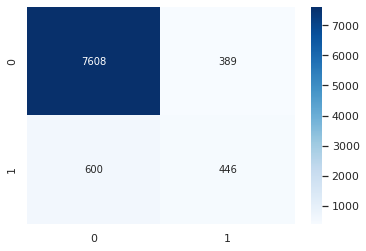
\includegraphics[width=0.5\textwidth]{cm-categorico.png}}
\end{figure}

\begin{figure}[H]
    \centerline{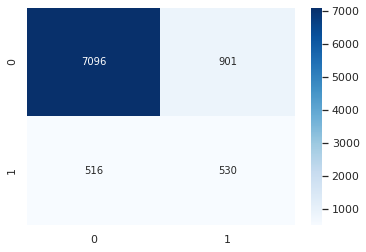
\includegraphics[width=0.5\textwidth]{cm-gaussiano.png}}
\end{figure}


\section{Análise dos Resultados}

\section{Conclusões e Discussões}




\bibliography{mybib}
\nocite{*}
\bibliographystyle{IEEEtran}
\end{document}
